\documentclass{standalone}
\usepackage{tikz}
\usepackage{amsmath}

\begin{document}

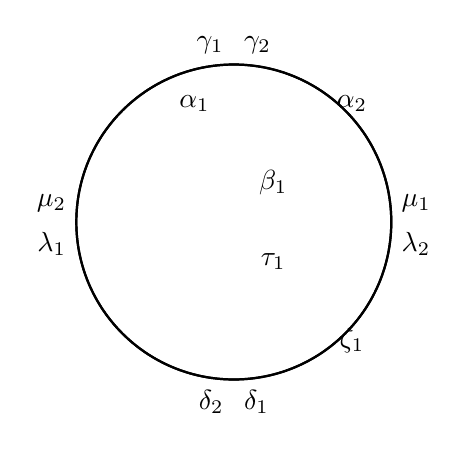
\begin{tikzpicture}

% First spherical linkage
\draw[thick]
    (0,0) coordinate (A) node[below left] {$\lambda_1$}
    to[out=90,in=180] (2,2) coordinate (B) node[above left] {$\gamma_1$}
    to[out=0,in=90] (4,0) coordinate (C) node[above right] {$\mu_1$}
    to[out=270,in=0] (2,-2) coordinate (D) node[below right] {$\delta_1$}
    to[out=180,in=270] (A);

% Second spherical linkage
\draw[thick]
    (4,0) coordinate (E) node[below right] {$\lambda_2$}
    to[out=90,in=0] (2,2) coordinate (F) node[above right] {$\gamma_2$}
    to[out=180,in=90] (0,0) coordinate (G) node[above left] {$\mu_2$}
    to[out=270,in=180] (2,-2) coordinate (H) node[below left] {$\delta_2$}
    to[out=0,in=270] (E);

% Labels for angles and gaps
\node at (1.5,1.5) {$\alpha_1$};
\node at (2.5,0.5) {$\beta_1$};
\node at (2.5,-0.5) {$\tau_1$};
\node at (3.5,1.5) {$\alpha_2$};
\node at (3.5,-1.5) {$\zeta_1$};

\end{tikzpicture}

\end{document}